
% \begin{eqa}[htbp] 
% 	\centering
% 	$ \sigma_F = ma $
% 	\caption{A photo} 
% \end{eqa}
% \begin{eqa}[htbp] 
% 	\centering
% 	$ \sigma_F = ma $
% 	\caption{A photo} 
% \end{eqa}
% \begin{figure}[htbp]
% 	\centering
% 	\includegraphics[scale=0.5]{test_image.jpg}
% 	\caption{ภาพใหม่}
% 	\label{fig:x cubed graph}
% \end{figure}
% จากรูปที่ {\ref{fig:x cubed graph}} จะเห็นว่า

% \begin{figure}[htbp]
% 	\centering
% 	\begin{subfigure}[b]{0.3\textwidth}
% 		\centering
% 		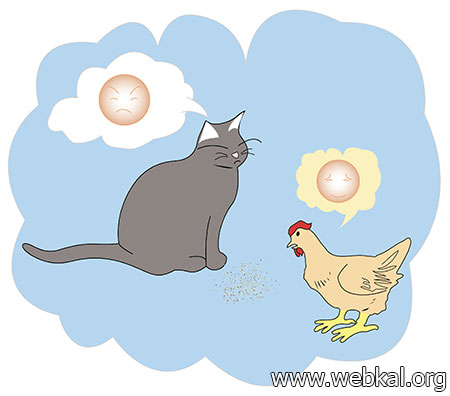
\includegraphics[width=\textwidth]{graph1.jpg}
% 		\caption{$y=x$}
% 		\label{fig:y equals x}
% 	\end{subfigure}
% 	\hfill
% 	\begin{subfigure}[b]{0.3\textwidth}
% 		\centering
% 		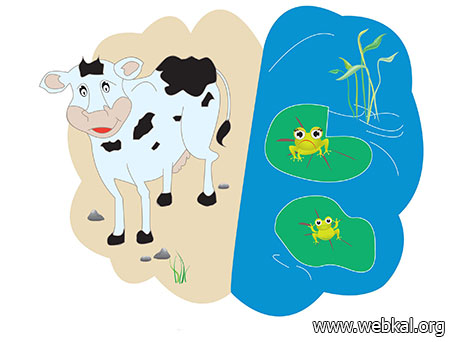
\includegraphics[width=\textwidth]{graph2.jpg}
% 		\caption{$y=3sinx$}
% 		\label{fig:three sin x}
% 	\end{subfigure}
% 	\hfill
% 	\begin{subfigure}[b]{0.3\textwidth}
% 		\centering
% 		
\includegraphics[width=\textwidth]{graph3.jpg}
% 		\caption{$y=5/x$}
% 		\label{fig:five over x}
% 	\end{subfigure}
% 	\caption{Three simple graphs}
% 	\label{fig:three graphs}
% \end{figure}

% \begin{table}[htbp]
% 	\centering
% 	\begin{tabular}{l | l | l}
% 		A & B & C \\
% 		\hline
% 		1 & 2 & 3 \\
% 		4 & 5 & 6 
% 	\end{tabular}
% 	\caption{very basic table}
% 	\label{tab:abc}
% \end{table}

% \begin{table}[htb]
% 	\begin{subtable}[h]{0.45\textwidth}
% 		\centering
% 		\begin{tabular}{l | l | l}
% 			Day   & Max Temp & Min Temp \\
% 			\hline \hline
% 			Mon   & 20       & 13       \\
% 			Tue   & 22       & 14       \\
% 			Wed   & 23       & 12       \\
% 			Thurs & 25       & 13       \\
% 			Fri   & 18       & 7        \\
% 			Sat   & 15       & 13       \\
% 			Sun   & 20       & 13       
% 		\end{tabular}
% 		\caption{First Week}
% 		\label{tab:week1}
% 	\end{subtable}
% 	\hfill
% 	\begin{subtable}[h]{0.45\textwidth}
% 		\centering
% 		\begin{tabular}{l | l | l}
% 			Day   & Max Temp & Min Temp \\
% 			\hline \hline
% 			Mon   & 17       & 11       \\
% 			Tue   & 16       & 10       \\
% 			Wed   & 14       & 8        \\
% 			Thurs & 12       & 5        \\
% 			Fri   & 15       & 7        \\
% 			Sat   & 16       & 12       \\
% 			Sun   & 15       & 9        
% 		\end{tabular}
% 		\caption{Second Week}
% 		\label{tab:week2}
% 	\end{subtable}
% 	\caption{Max and min temps recorded in the first two weeks of July}
% 	\label{tab:temps}
% \end{table}

% \clearpage



% \bibliographystyle{ieeetr}
% \bibliography{references/references}
% fdsakfodsaofkdaosf
% \bibentry{einstein}
% \bibentry{knuthwebsite}
% \bibentry{latexcompanion}
% \citep{einstein}
% \citep{knuthwebsite}
% \citep{latexcompanion}
% fdaslfdlsa;flsa;d

\begin{figure}[htb]
	\centering
    \includegraphics[scale=0.5]{chapter1/images/test_image.jpg}
    \caption{ภาพใหม่}
\end{figure}
\begin{table}[htb]
	\centering
	\begin{tabular}{l | l | l}
		A & B & C \\
		\hline
		1 & 2 & 3 \\
		4 & 5 & 6 
	\end{tabular}
	\caption{very basic table}
	\label{tab:abc}
\end{table}
\begin{table}[htb]
	\centering
	\begin{tabular}{l | l | l}
		A & B & C \\
		\hline
		1 & 2 & 3 \\
		4 & 5 & 6 
	\end{tabular}
	\caption{very basic table}
	\label{tab:abc}
\end{table}
\begin{table}[htb]
	\centering
	\begin{tabular}{l | l | l}
		A & B & C \\
		\hline
		1 & 2 & 3 \\
		4 & 5 & 6 
	\end{tabular}
	\caption{very basic table}
	\label{tab:abc}
\end{table}
\begin{table}[htb]
	\centering
	\begin{tabular}{l | l | l}
		A & B & C \\
		\hline
		1 & 2 & 3 \\
		4 & 5 & 6 
	\end{tabular}
	\caption{very basic table}
	\label{tab:abc}
\end{table}
\begin{table}[htb]
	\begin{subtable}[h]{0.45\textwidth}
		\centering
		\begin{tabular}{l | l | l}
			Day   & Max Temp & Min Temp \\
			\hline \hline
			Mon   & 20       & 13       \\
			Tue   & 22       & 14       \\
			Wed   & 23       & 12       \\
			Thurs & 25       & 13       \\
			Fri   & 18       & 7        \\
			Sat   & 15       & 13       \\
			Sun   & 20       & 13       
		\end{tabular}
		\caption{First Week}
		\label{tab:week1}
	\end{subtable}
	\hfill
	\begin{subtable}[h]{0.45\textwidth}
		\centering
		\begin{tabular}{l | l | l}
			Day   & Max Temp & Min Temp \\
			\hline \hline
			Mon   & 17       & 11       \\
			Tue   & 16       & 10       \\
			Wed   & 14       & 8        \\
			Thurs & 12       & 5        \\
			Fri   & 15       & 7        \\
			Sat   & 16       & 12       \\
			Sun   & 15       & 9        
		\end{tabular}
		\caption{Second Week}
		\label{tab:week2}
	\end{subtable}
	\caption{Max and min temps recorded in the first two weeks of July}
	\label{tab:temps}
\end{table}
\begin{table}[htb]
	\centering
	\begin{tabular}{l | l | l}
		A & B & C \\
		\hline
		1 & 2 & 3 \\
		4 & 5 & 6 
	\end{tabular}
	\caption{very basic table}
	\label{tab:abc}
\end{table}

\begin{table}[htb]
	\begin{subtable}[h]{0.45\textwidth}
		\centering
		\begin{tabular}{l | l | l}
			Day   & Max Temp & Min Temp \\
			\hline \hline
			Mon   & 20       & 13       \\
			Tue   & 22       & 14       \\
			Wed   & 23       & 12       \\
			Thurs & 25       & 13       \\
			Fri   & 18       & 7        \\
			Sat   & 15       & 13       \\
			Sun   & 20       & 13       
		\end{tabular}
		\caption{First Week}
		\label{tab:week1}
	\end{subtable}
	\hfill
	\begin{subtable}[h]{0.45\textwidth}
		\centering
		\begin{tabular}{l | l | l}
			Day   & Max Temp & Min Temp \\
			\hline \hline
			Mon   & 17       & 11       \\
			Tue   & 16       & 10       \\
			Wed   & 14       & 8        \\
			Thurs & 12       & 5        \\
			Fri   & 15       & 7        \\
			Sat   & 16       & 12       \\
			Sun   & 15       & 9        
		\end{tabular}
		\caption{Second Week}
		\label{tab:week2}
	\end{subtable}
	\caption{Max and min temps recorded in the first two weeks of July}
	\label{tab:temps}
\end{table}
\clearpage